\documentclass[10pt, preprint]{aastex}
\usepackage{fullpage,enumitem,amsmath,amssymb,graphicx, subfigure}
\usepackage{graphicx} % This is a package for including graphics in your solution.
\usepackage{tikz}
\usepackage{listings}
\usetikzlibrary{automata, positioning, arrows}
\DeclareMathOperator*{\argmax}{arg\,max}

\tikzset{
	->,
	>=stealth'
}


\begin{document}

\begin{center}
{\Large CS 6466 2 Chains: Miner Dynamics Across Blockchains}


\begin{tabular}{lr}
Email: & wdaviau@protocol.ai \\
CUNet ID: & wtd37 \\
Name: & Wyatt Daviau \\
Date: & March 25th 2018 \\
\end{tabular}
\end{center}


\section{Abstract}
We model the scenario where two blockchains have the same proof of work hash function and therefore miners can switch among chains at will.  We devise a principled simple strategy for choosing among competing blockchains that miners can follow.  We demonstrate that this strategy is profitable throughout a large region of the considered parameter space and classify different regions of the parameter space based on the behavior of miners following this profitable strategy.  We present an analysis of historical BTC / BCH data in light of our 

Furthermore we investigate what an optimal switching strategy would look like if miners can make reasonable predictions about the future.  We also propose a candidate strategy for a blockchain designed to compete with an existing chain for hash power without flooding the market for its native token by minting coins at an excessive rate.

\section{Introduction}
The recent Bitcoin Cash (BCH) fork of the Bitcoin (BTC) blockchain serves as an example of a relatively powerful fork of a blockchain network.  Such forks naturally lead to multiple blockchain networks using the same proof of work function.  In such a world "mercenary" miners can potentially increase profits by dynamically switching their hash power across chains.  Recent events have shown that this can have detrimental effects on the networks involved [1] due to drastic changes in profitability among chains and a slow response to large changes in hashrate that trace back to details in bitcoin's difficulty adjustment algorithm.

The goal of our analysis is to study the scenario in which miners are willing to switch between two blockchains that run the same difficulty adjustment protocol to maximize their net profits.  We define a plausible parametrization of this system and then study potential chain-switching strategies that miners might employ in an attempt to increase their profits.  We begin by trying to understand the profitability over time of what we deemed the "greedy mercenary" approach, and the regions in which this leads to stable and unstable hash power allocations across chains.  From first principles we come up with a simple metric mercenary miners could use to decide on the best chain and end up rediscovering the so-called "Difficult Adjustment Reward Index" or DARI that miners actually use during operation. 

[Ahaan discussion of further optimal algorithms or optimality of greedy mercenary]

We model the system consisting of two chains both running BTC's difficulty adjustment protocol but sweeping different reward fractions, "loyal" hashrates and mercenary hashrate.  Based on our model we introduce a simple visualization for the stability characteristics of different points in the parameter space and an associated prediction function determining whether a point in the parameter space will be unstable. We built simple simulation and analysis frameworks for generating and interpreting data representing execution of these systems in the presence of mercenary miners following the greedy strategy.  Leveraging these frameworks we present a view into the different stability regions of the parameter space and reach the conclusion that the greedy mercenary mining strategy is profitable throughout a wide section of the parameter space.  We confirm our theoretical prediction of the instability region concluding that in the BTC / BTC difficulty adjustment case the region of instability in the parameter space is significant and  [impacts the transaction throughput of both systems TODO analysis function and figure quantifying this]. 

[ Arnesh + Wyatt TODO BCH / BTC, BCH / BCH simulation results would be a great addition to this paper and seems within reach with one week remaining ] 

[ Arnesh + Ahaan analysis of historical data sets, maybe this should be skipped as DARI is already plotted by fork.lol? ]


\section{Model and Assumptions}
We make many simplifying assumptions when modeling this system.  The goal is to make enough assumptions to keep analysis tractable while at the same time parameterizing the problem in a way that gives insight to real systems of competing blockchains, and paves the way for more advanced modeling.  The following are global system assumptions 
\begin{enumerate}
\item
There are two chains in the system, chain 1 and chain 2.  Both chains use the same proof of work and difficulty adjustment algorithm as the Bitcoin protocol [TODO when BCH difficulty is added in this will change]
\item
Each chain rewards miners with a coinbase transaction that pays out tokens to the miner that solves the block puzzle.  Additionally miners are rewarded by the transaction fees tied to the transactions serialized in the blocks.  We assume that the value of the total reward (in, say USD) of chain 1 is a constant $f_1$ and the value of the token of chain 2 is a constant $f_2$.  We do not account for variations in transaction fees or reductions in the coinbase payout in this analysis.  Only the ratio of these two parameters $\frac{f1}{f2}$ is relevant in our analysis.
\item
We model the total hash rate of the system as $H$ (hashes / second) and assume that it does not change over the period of analysis in question.  
\item
Fractions of the hashpower belong to three different entities, $\alpha$, $\beta_1$, $\beta_2$.  $\alpha$ + $\beta_1$ + $\beta_2$ = 1.
\item
We assume a fraction $\alpha$ of the hash power, from here on out called the mercenary miners, is willing to switch between chains in order to make a profit.  In the case of our analysis of the Greedy Mercenary Mining strategy we do NOT need to make the assumption that the hashpower $\alpha$ belongs to a single pool.  This is elaborated further in the following section.
\item
$\beta_1$ and $\beta_2$ corresponding to miners who are loyal to chains 1 and 2 respectively.  These hashpower fractions do not move from their respective chains regardless of the profitability of switching.  We need not consider the hash power of $\beta_i$ as belonging to a single pool.
\item
The difficulty of each chain is adjusted every $b$ blocks.  The time it takes for $b$ blocks to be mined in epoch $i$ = $\Delta_i$.  To calculate the difficulty adjustment the protocol specifies that: $d_{i+1} = \frac{ d_i \cdot b \cdot t_{\text{target}} }{ \Delta_i}$, as in bitcoin.  The target is 600s.

\item
We assume the system begins in a steady state where the difficulty of each chain reflects the initial allocation of the hash power.  The mercenary miners begin by mining on chain 1.  Throughout the analysis chain 1 is given the asymetric advantage that $\frac{f1}{f2} \leq 1$
\end{enumerate}

\subsection{Calculating the initial difficulty}

From assumption (8) above we can calculate the initial difficulty, which is an initial condition needed by the simulation framework.  We include the derivation here because the discussion is relevant for the subsequent derivation of the switching criterion for the greedy mining strategy.  

The following discussion applies to both chains and examines chain 1 without loss of generality.  By our steady state assumption that the mining epoch before the period of history in which our analysis takes place lasted exactly $(600 s)(b)$.  The number of hashes tried until a block is successfully mined follows a geometric distribution and by the properties of this distribution the inverse of the probability of one success is equal to the mean number of hashes until success.  Given our steady state condition and initial allocation we have the following relation
$$
600 H(\alpha+ \beta_1) = \frac{1}{p}
$$
Where $p$ is the probability of one hash solving the block puzzle.
Recall that the difficulty of a chain is given by
$$
\frac{F_{\text{max}}}{F}
$$
where $F$ is the threshold value below which a block with the given hash solves the puzzle.  As the range of the hash function used in the chain puzzle is binary strings of 256 characters, $p = \frac{F}{2^{256}}$ and therefore
\begin{align*}
600 H(\alpha + \beta_1) &= \frac{2^{256}}{F}\\
600 H(\alpha + \beta_1)F_{\text{max}} &= \frac{2^{256}F_{\text{max}}}{F}\\
\frac{600 H(\alpha + \beta_1)F_{\text{max}} }{2^{256}} &= d_{10}
\end{align*}
where $d_{1i}$ is the difficulty of chain 1 in the $i$th adjustment period of chain 1.  Factoring out constants we have
\begin{align*}
\mathcal{D} &= \frac{HF_{\text{max}} }{2^{256}}\\
d_{10} &= 600\mathcal{D} (\alpha + \beta_1)\\
d_{20} &= 600\mathcal{D} (\beta_2)\\
\end{align*}

\section{The Greedy strategy}
What happens if the switching miner decides to maximize for profit with a simple greedy algorithm, that is, an algorithm making no predictions about the future hash allocations or reward schedules of the two chains?  The sensible way to do this is to compare the expected rate of reward on both chains at any time.  We now show that the simplified form of the expected reward rate at difficulty adjustment period $i$ is simply $$\frac{f_1}{d_i} \cdot \alpha$$.  Let $\mathcal{E}_{ij}[T]$ be the expected time to mine a block on chain $j$ in difficulty period $i$.  The expectation is taken over the randomness in solving hash puzzles while assuming the difficulty $d_i$ is known.  To start we assume that there is only one mercenary mining pool with hash power $\alpha$, and later show how to relax this assumption.

As we saw in the last section the expected time to find a block can be related to the chain difficulty:
\begin{align*}
& \mathcal{E}_i[T] (\alpha + \beta_j)H = \frac{1}{p} \\
& \mathcal{E}_i[T] (\alpha + \beta_j)H = \frac{2^{256}}{F_{i}}\\
& \mathcal{E}_i[T] (\alpha + \beta_j)H = d_{ij} \frac{2^{256}}{F_{\text{max}}}\\
& \mathcal{E}_i[T] = \frac{d_{ij}}{\mathcal{D}(\alpha + \beta_j)} \\
\end{align*}

Now we can calculate the expected profit to mine on chain $j$ during difficulty period $i$ as follows
\begin{align*}
& \frac{\text{reward per block} }{\text{expected time per block}} \cdot (\text{expected winning fraction}) \\
&= \frac{f_j}{\mathcal{E}_i[T]} \cdot \frac{\alpha}{\alpha + \beta_j}\\
&= \frac{f_j \cdot \mathcal{D}(\alpha + \beta_j)}{d_{ij}} \cdot \frac{\alpha}{\alpha + \beta_j}\\
&= \frac{f_j \cdot \mathcal{D}\alpha}{d_{ij}}\\
\end{align*}

As $\mathcal{D}$ and $\alpha$ appear in the profit rates of both chains, the greedy mercenary mining strategy checks the difficulty of the current period on each chain $d_1$ and $d_2$ and mines on chain
$$\argmax{\frac{f_j}{d_j}}$$

In our simplifying model the fractional reward does not change and therefore the miner will only benefit from switching when one of the chains adjusts its difficulty.  When one profit rate is strictly greater than the other the mercenary miner does not stand to benefit in the short term from allocating some hashpower to the less profitable chain so all $\alpha$ goes to the most profitable chain.  In the case both profit rates are equal the greedy mercenary miner chooses a chain at random. 

A key observation regarding the profit rate is that while changes in the block reward and difficulty values influence which chain is most profitable, the addition or subtraction of other mercenary hash power within the same period does not affect the outcome on expectation.  Intuitively this is because the expected rate of block emission changes exactly inversely proportionally to the change in the expected winning fraction of a given mining pool.  This is encoded in the algebra above by the appearance of $(\alpha + \beta_j)$ in both the numerator and denominator.  As a consequence the choices of one greedy mercenary miner is not affected by the choices of another, at least in our simplifying fixed reward model.  This means that we can model $\alpha$ as the hash power of ALL mercenary miners, and that our results are easier to apply to this more general case.

\subsubsection{Application to real mining}
After deriving our simple greedy strategy independently, it turns out that our algorithm is apparently used by real-life mercenary miners, or as they are sometimes called "chain-hoppers".  Our switching criterion is known as the Difficulty Adjustment Reward Index by miners in the BCH community and is tracked by at least one BCH analytics site [2].

\subsubsection{Theoretical Analysis}
[TODO -- Figure one needs axes revamp (0 to 1 not 100) and should be taken over a finer grained step sizes to get smoother plots.  Also we should get rid of pplot for this graph]
\begin{figure}
	\centering
	\subfigure[$\alpha=0.01$]{
		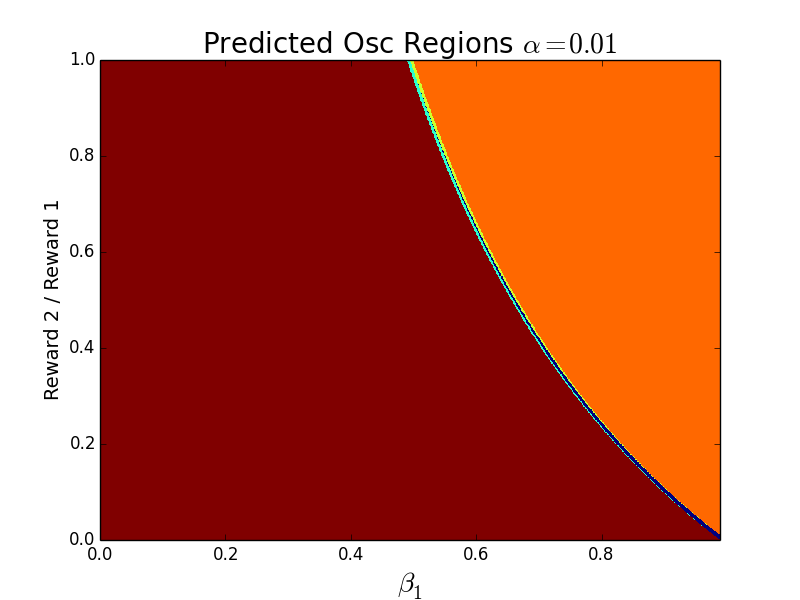
\includegraphics[width=0.3\linewidth]{simulations/resources/predicted-osc-regions-alpha=0-01.png}
		\label{fig:theo}
		}
	\qquad
	\subfigure[$\alpha=0.05$]{
		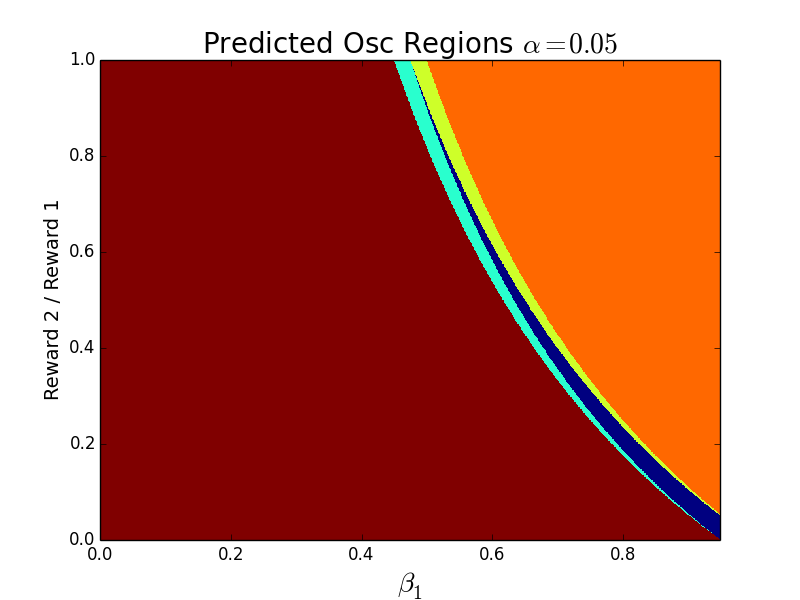
\includegraphics[width=0.3\linewidth]{simulations/resources/predicted-osc-regions-alpha=0-05.png}
		\label{fig:theo}
		}
	\qquad
	\subfigure[$\alpha=0.1$]{
		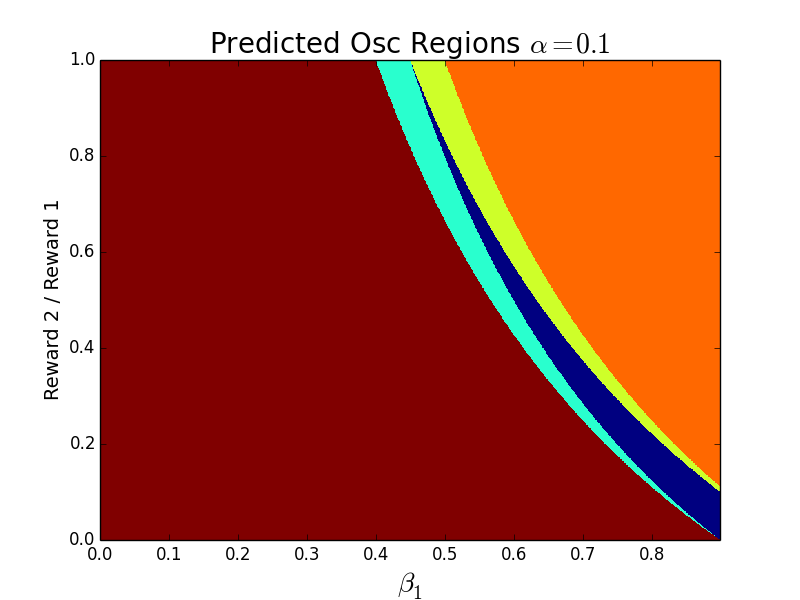
\includegraphics[width=0.3\linewidth]{simulations/resources/predicted-osc-regions-alpha=0-1.png}
		\label{fig:theo}
		}
	\qquad
	\subfigure[$\alpha=0.3$]{
		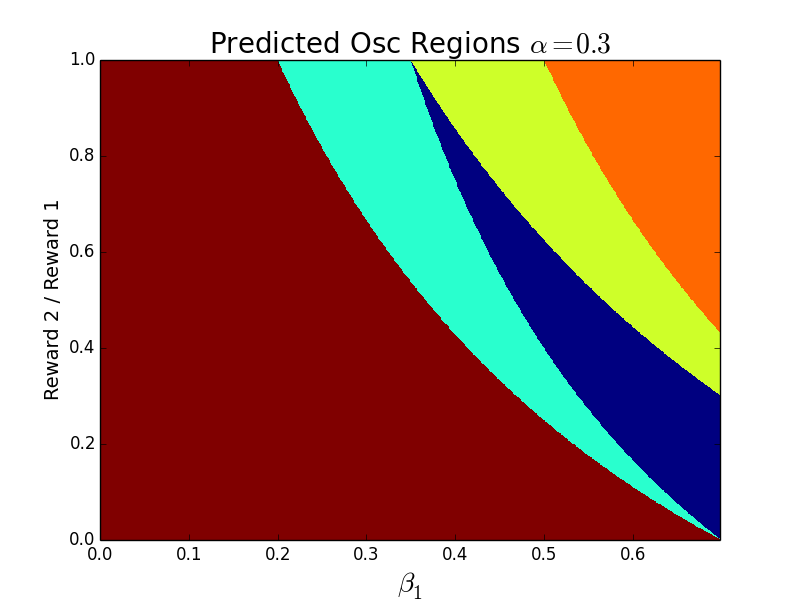
\includegraphics[width=0.3\linewidth]{simulations/resources/predicted-osc-regions-alpha=0-3.png}
		\label{fig:theo}
		}		
	\caption{Orderings over different regions of parameter space. Index -- Red: (1), Orange: (2), Cyan: (3), Blue: (4), Yellow: (5)}
\end{figure}

Given the mechanism of the greedy mercenary mining strategy and the properties of the protocol difficulty, one useful characterization of a two chain system is the ordering of the four values: 
$$
\frac{f_2}{\alpha + \beta_2}, \frac{f_2}{\beta_2}, \frac{f_1}{\alpha + \beta_1}, \frac{f_1}{\beta_1}
$$
In a rough sense the value $\frac{f_j}{\alpha + \beta_j}$ can be thought of as the least profitable expected profit rate and $\frac{f_j}{\beta_j}$ the most profitable expected profit rate on chain $j$.  This is because the difficulty is distributed about a mean proportional to the average hash rate on the previous interval and the greatest and least possible such average hash rates are $\alpha + \beta_j$ and $\beta_j$ respectively.  The proportionality constants are ignored here because they are identical across each ratio and don't affect the ordering.  

Due to the constraints $\frac{f_j}{\alpha + \beta_j} < \frac{f_j}{\beta_j}$, there are 6 possible orderings of these values: [TODO -- make this look less complicated by assigning visualizations to each of the four values as done in written examples.  Also putting on the number line might be nice]
\begin{enumerate}
\item
$\frac{f_2}{\alpha + \beta_2} < \frac{f_2}{\beta_2} < \frac{f_1}{\alpha + \beta_1} < \frac{f_1}{\beta_1}$
\item
$\frac{f_1}{\alpha + \beta_1} < \frac{f_1}{\beta_1} < \frac{f_2}{\alpha + \beta_2} < \frac{f_2}{\beta_2} $
\item
$\frac{f_2}{\alpha + \beta_2} < \frac{f_1}{\alpha + \beta_1} < \frac{f_2}{\beta_2} < \frac{f_1}{\beta_1}$
\item
$\frac{f_1}{\alpha + \beta_1} < \frac{f_2}{\alpha + \beta_2} < \frac{f_1}{\beta_1} < \frac{f_2}{\beta_2}$
\item
$\frac{f_1}{\alpha + \beta_1} <  \frac{f_2}{\alpha + \beta_2} < \frac{f_2}{\beta_2} <  \frac{f_1}{\beta_1} $
\item
$ \frac{f_2}{\alpha + \beta_2} <  \frac{f_1}{\alpha + \beta_1} < \frac{f_1}{\beta_1}  < \frac{f_2}{\beta_2} $
\end{enumerate}

Any point in the parameter space defined by: $(\alpha, \beta_1, \beta_2, f_1, f_2)$ satisfies one of these orderings (or is on the boundary between them in the case of equality).  The ordering assigned to a given system should be an indicator of whether or not hash power oscillations can be expected between chains in this system.  

We do not expect oscillations for systems with orderings (1) or (2).  In these cases one chain's lowest profitability rate is higher than the other chain's highest rate and and no mercenary greedy miner would ever switch to the less profitable chain.  

We expect oscillations in the remaining orderings (3), (4), (5), (6).  Orderings (5) and (6) result in oscillations with a single mode.  In ordering (5) when the difficulty of chain 1 is at its lowest point then mercenaries flock to chain 1, but when the difficulty is at its maximum value they move to chain 2, and symmetrically for ordering (6).  Orderings (3) and (4) are a bit more complex.  Like ordering (5), in ordering (3) when chain 1's difficulty is at its lowest mercenaries move to chain 1.  However mercenaries do not always move to chain 2 when chain 1's difficulty is at its max value, this now depends on the difficulty of chain 2 as well.  Figure 1 plots the ordering corresponding to each point in parameter space, hypothesizing the region of instability. 

Note that there are a few simplifications here.  Most obviously because difficulty tracks with block discovery time which is not deterministic, the values in the orderings do not perfectly correspond to the actual values that will be compared by the mercenary miners during system execution.  In reality the difficulty adjustment alogirthm samples the ordering values in a distribution surrounding the values listed here.  This could lead to different systems in the parameter space displaying different orderings at different difficulty adjustment periods.  For example a system with ordering (2) could have middle points very close such that after a given adjustment $\frac{f_1}{\beta_1} >\frac{f_2}{\alpha + \beta_2}$, giving the system ordering (4).

Furthermore in the case where miners switch in the middle of one of chain $j$'s adjustment periods due to a profitability adjustment triggered by the other chain, then the average hash rate, and therefore expected difficulty value on chain $j$, in the next period will be between the two extreme values that appear in this ordering.  Again this can change the true ordering of the chain during execution and lead to behavior not predicted by figure 1.  We simulate mining on a two chain system and describe the results in the next section to measure the true oscillation regions that emerge in light of the above two complications.

\section{Simulations}
To confirm our hypotheses with greater confidence we built a small simulation and analysis framework in under 600 lines of python.  This simulation framework generates and saves data sets recording data for each difficulty adjustment period.  Sweeps are made to record this data throughout the parameter space.  The analysis framework reads data files and applies filters across subsections of data to flexibly generate values suitable for plotting from the raw data.  These techniques provided us with clear visualizations of the profitability and instability of different regions of the parameter space.

\subsection{Methodology}
Our code is located on github at: https://github.com/ZenGround0/2Chainz
\subsubsection{Simulation Framework and Sweeps}
The simulation framework generates a blockchain history from input parameters $\alpha$, $\beta_j$, $f_j$, $d_{0j}$, $b$ and $t_{\text{target}}$.  It mines blocks on each chain with a time drawn from an exponential distribution, records difficulty adjustments and places the mercenary hash power on the chain given by the strategy defined in section 5.  Each period of time between switching events is recorded as 2 4 tuples.  Each chain records (time, blocks mined, difficulty, hash power on chain)

We broke our parameter space into 3 standard degrees of freedom: $\alpha$, $\beta_1$, and $\frac{f2}{f1}$.  We swept price fractions and $\beta$ values at precision of 0.01 and ran each such sweep with alpha values of 0.01, 0.05, 0.1, 0.2, 0.3.  We began by running 5 trials for each point and running for 100 difficulty adjustments.  Datasets are persisted to disk as csv files and each such sweep generates about 3 GB of data.

 We performed a simple statistical analysis on the mean and standard deviations of the oscillation count data set to measure how much greater a sample size we should take to increase our confidence in the results.  The test showed that apart from a small subset of points well understood to be highly variant, 5 trials was more than enough to be 90\% confident in our samples.  Furthermore only 5 more trials would be sufficient to get to 90\% confidence in the small subset of high variance points.

[TODO not necessary but we could potentially justify far fewer difficulty adjustment periods to get meaningful data (expected profit, oscillations / hash power residency).  This would take some initial work but would result in much faster and probably more principled simulations.  Initial work would center around plotting out individual runs and looking for convergence patterns.  Alternatively coming up with a map function measuring a meaningful notion of convergence in the parameter space and running a normal plot job.  I am confident 100 runs is well past convergence, and also a little much given that it is 2 years of acutal time ]

\subsubsection{Analysis Framework}
We wrote a data processing and plotting script that leverages a simple map reduce framework to easily compose operations and make generation of plots easy to reason about.  We built a simple map reduce framework: the map function processes the data of a single trial's history and the reduce function aggregates together all of the values of all trials occurring at the same point in the parameter space.  The plots generated are of the entire parameter space sweep.  Each plot represents one value of $\alpha$, i.e. the combined hash rate of all mercenary miners.  The x-axis measures $\beta_1$, the hash rate loyal to the more powerful chain 1, and the y-axis measures the fraction $\frac{f2}{f1}$ between the values of 0 and 1.

[TODO plots of individual runs.  This is a precursor for the previous TODO.  It is not necessary but might help present results + is necessary for reducing the number of difficulty adjustments in simulations in a principled way.  Also this is a pretty simple endeavor ~2 hours and it could shave lots and lots of time from simulations this week]
\subsection{Results}
Figure 2 shows the mean number of oscillations across all trials at each point swept for the simulated model.  The results are close to those predicted in Figure 1, but the oscillation regions extend past the predicted boundaries due to the element of randomness complicating the true ordering of profit rates between chains discussed in 5.0.2.  As the hash power of mercenary miners increases, a larger region of the parameter space is unstable.
[TODO -- axes labeled right, perhaps nicer font and sizing for axes.  Title could be formatted better too but not essential]
\begin{figure}
	\centering
	\subfigure[$\alpha=0.01$]{
		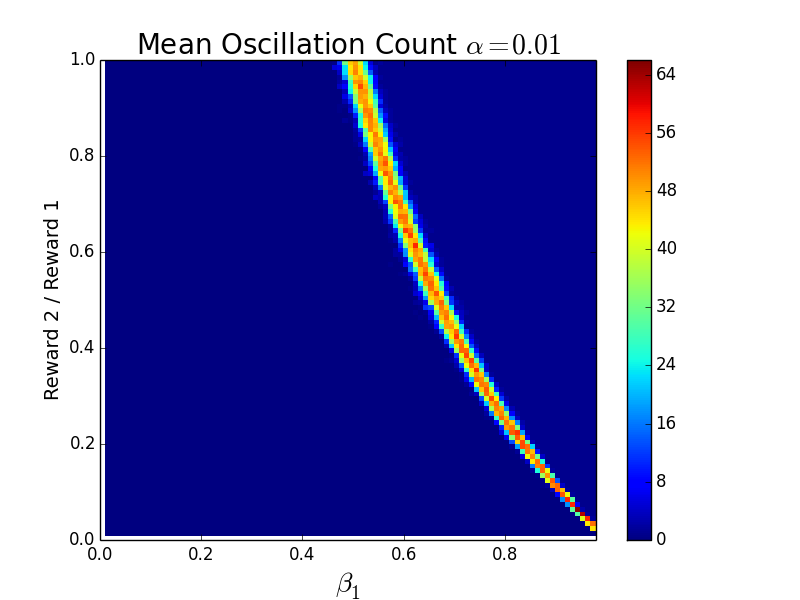
\includegraphics[width=0.25\linewidth]{simulations/resources/mean-oscillations-alpha=0-01.png}
		\label{fig:theo}
		}
	\qquad
	\subfigure[$\alpha=0.05$]{
		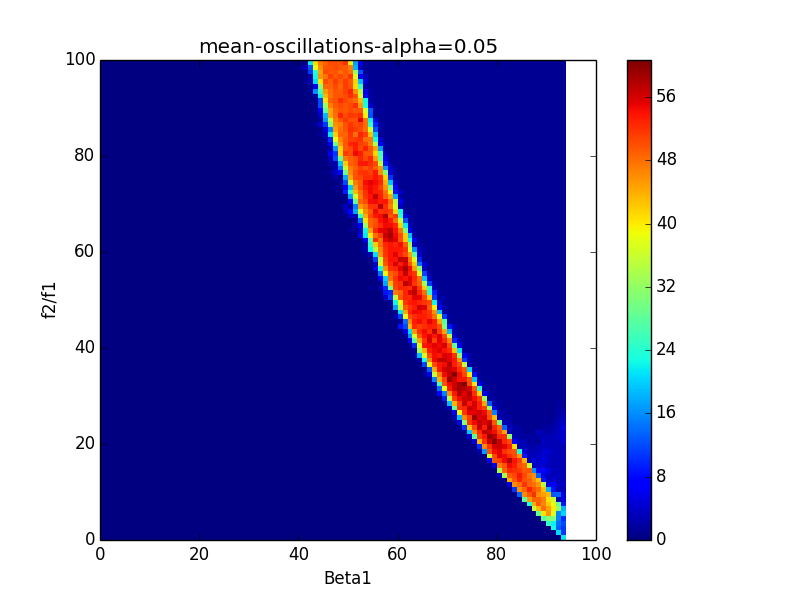
\includegraphics[width=0.25\linewidth]{simulations/resources/mean-oscillations-alpha=0-05.png}
		\label{fig:theo}
		}
	\qquad
	\subfigure[$\alpha=0.1$]{
		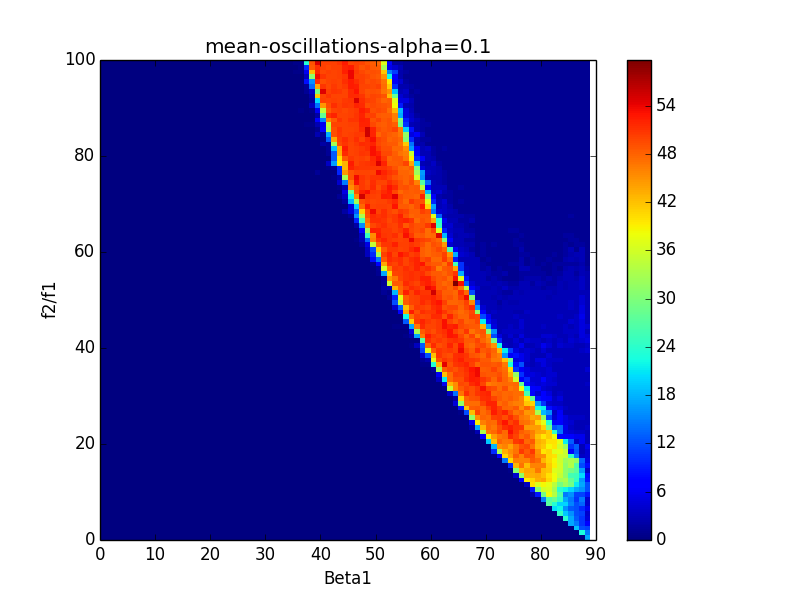
\includegraphics[width=0.25\linewidth]{simulations/resources/mean-oscillations-alpha=0-1.png}
		\label{fig:theo}
		}
	\qquad
	\subfigure[$\alpha=0.2$]{
		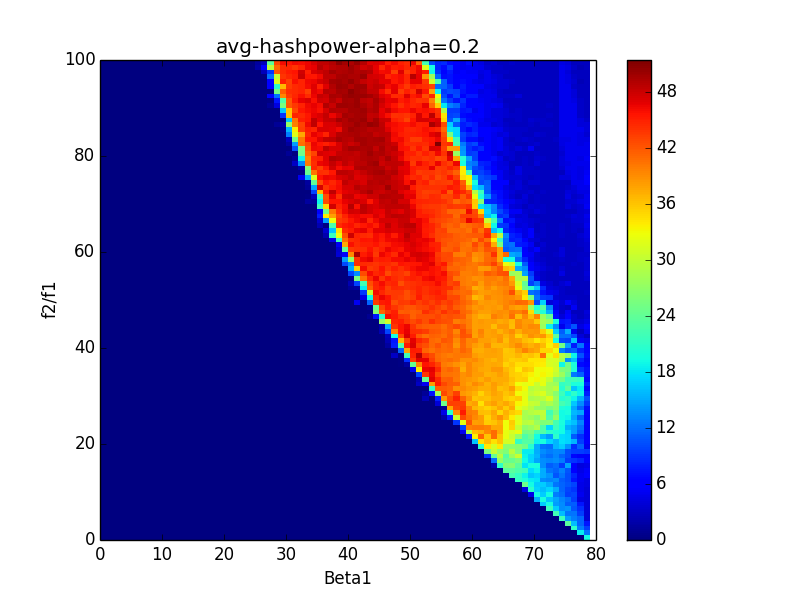
\includegraphics[width=0.25\linewidth]{simulations/resources/mean-oscillations-alpha=0-2.png}
		\label{fig:theo}
		}
	\qquad
	\subfigure[$\alpha=0.3$]{
		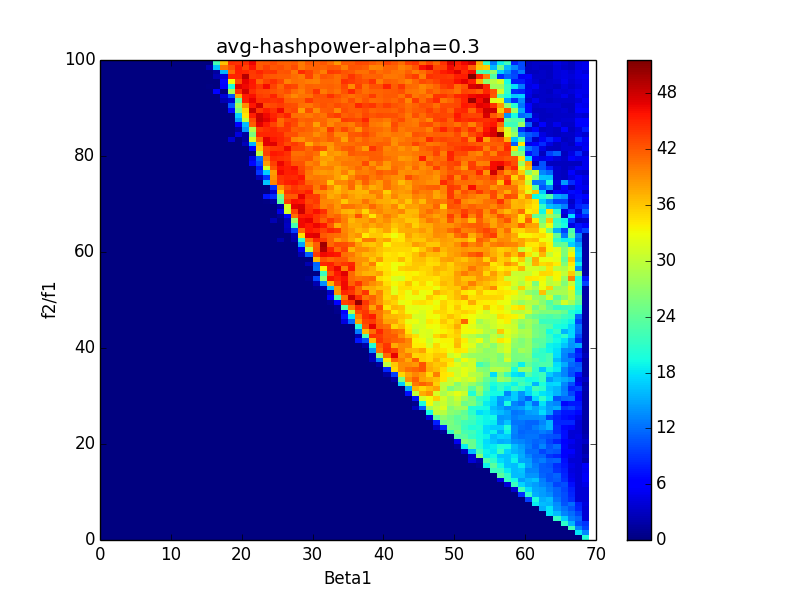
\includegraphics[width=0.25\linewidth]{simulations/resources/mean-oscillations-alpha=0-3.png}
		\label{fig:theo}
		}		
	\caption{Mean number of oscillations over 100 difficulty adjustment periods.  One oscillation occurs when the mercenary hash power switches between chains once.}
\end{figure}

[TODO -- remove the scale on the right from all, and fix axes]
Figure 3 marks in green regions where no oscillations occur in all trials (region 1), in red regions where only one oscillation from chain 1 to chain 2 occurs in all trials (region 2), and in blue regions where more than one oscillation occurs in at least one trial (region 3)
\begin{figure}
	\centering
	\subfigure[$\alpha=0.01$]{
		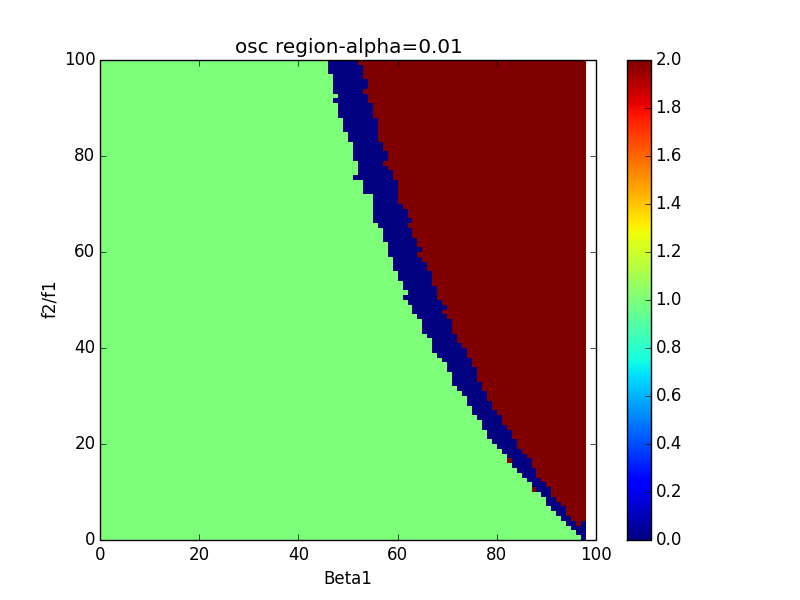
\includegraphics[width=0.25\linewidth]{simulations/resources/osc-region-alpha=0-01.png}
		\label{fig:theo}
		}
	\qquad
	\subfigure[$\alpha=0.05$]{
		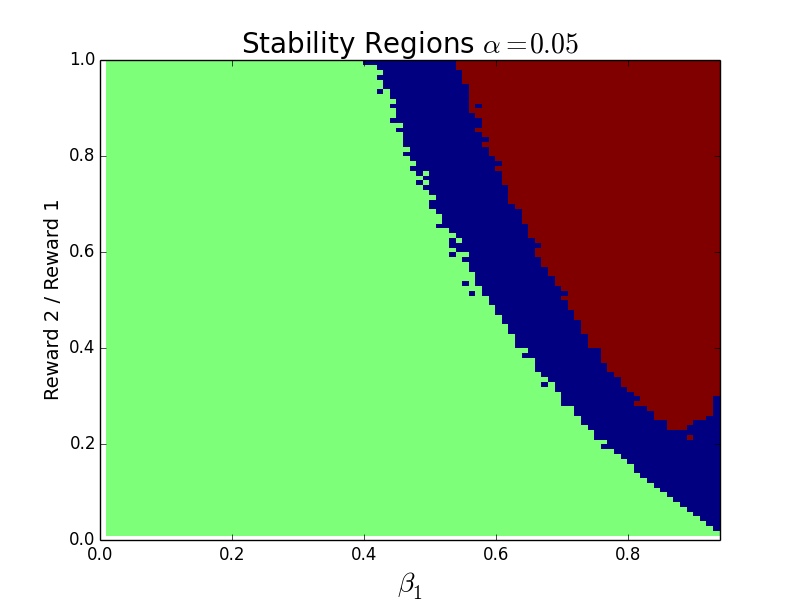
\includegraphics[width=0.25\linewidth]{simulations/resources/osc-region-alpha=0-05.png}
		\label{fig:theo}
		}
	\qquad
	\subfigure[$\alpha=0.1$]{
		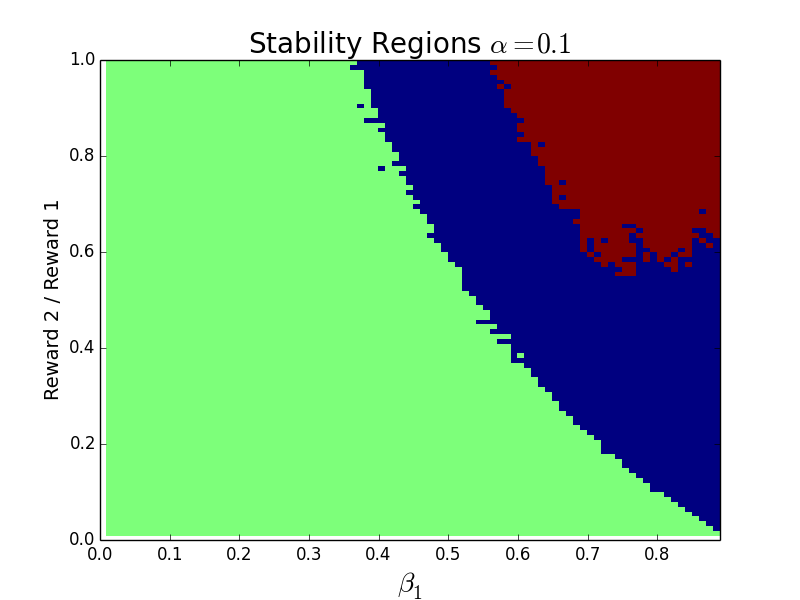
\includegraphics[width=0.25\linewidth]{simulations/resources/osc-region-alpha=0-1.png}
		\label{fig:theo}
		}
	\qquad
	\subfigure[$\alpha=0.2$]{
		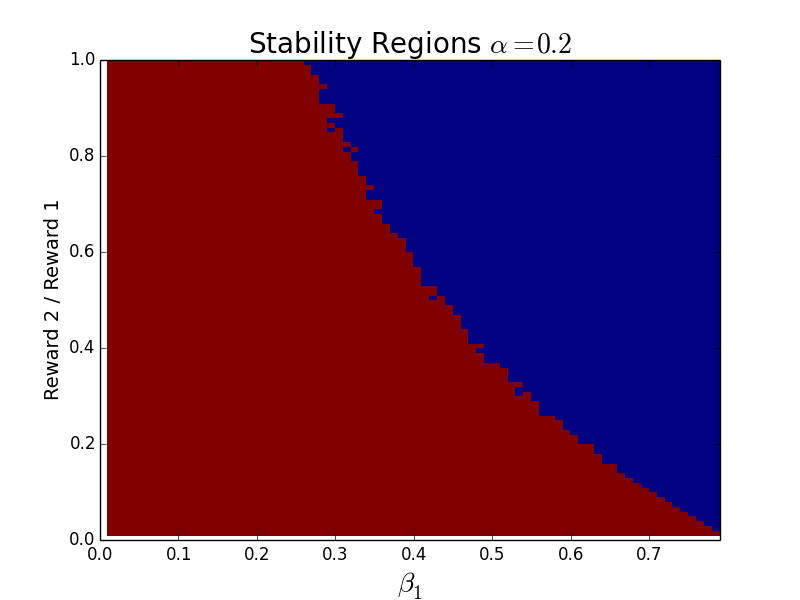
\includegraphics[width=0.25\linewidth]{simulations/resources/osc-region-alpha=0-2.png}
		\label{fig:theo}
		}
	\qquad
	\subfigure[$\alpha=0.3$]{
		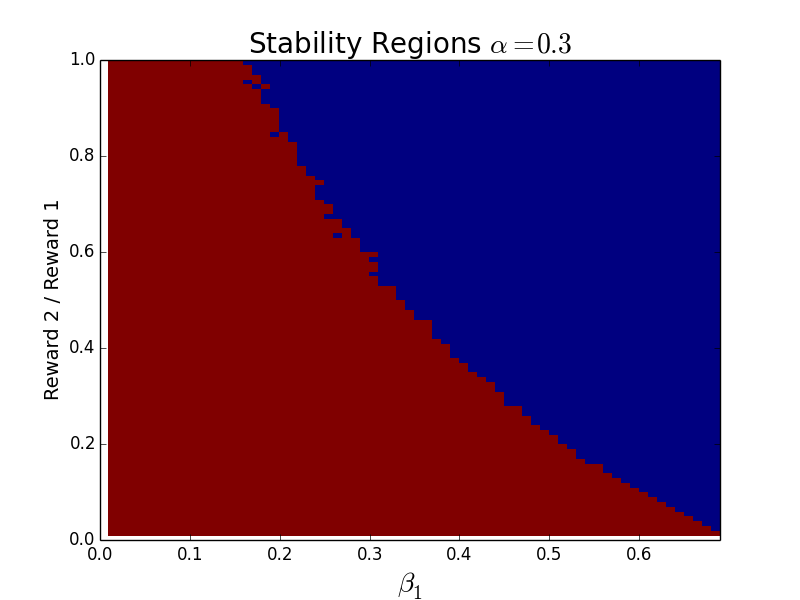
\includegraphics[width=0.25\linewidth]{simulations/resources/osc-region-alpha=0-3.png}
		\label{fig:theo}
		}		
	\caption{Different stability regions.  Chain 1 dominates in region 1 in green.  Chain 2 dominates in region 3 in red, oscillations occur in blue.  As alpha increases the region of instability consumes most of the parameter space.}
\end{figure}

[TODO -- fix axes]
Figure 4 shows the average expected profit of a mercenary following the greedy strategy taken over the simulation trials normalized by the expected profit if the mercenary hashrate had stayed on chain 1.  It is calculated by adding up $b_i \cdot \frac{\alpha}{\alpha + \beta_j} \cdot f_j$ for both chains $j=1,2$ for all periods $i$ where the mercenary hash rate is resident on that chain.  The profit is then normalized by dividing by the expected profit the mercenary miners would make if they had stayed on chain 1 over the same period of time.  

Note that the normalized profit is higher for smaller values of $\alpha$.  This can be explained intuitively by recognizing that when mercenary miners make up a smaller fraction of the total hash power of the system, their total fraction of power on chain 2 is relatively greater than their total fraction of power on chain 1.  Alternatively consider the power ratios on both chains
$$
\frac{ \frac{\alpha}{\alpha + \beta_2}}{\frac{\alpha}{\alpha + \beta_1}} = \frac{\alpha + \beta_1}{\alpha + \beta_2}\\ 
$$

When $\alpha, \beta_2 << \beta_1$ $\frac{\alpha + \beta_1}{\alpha + \beta_2} \approx \frac{\beta_1}{\beta_2}$.  When $\alpha \approx \beta_1$ $\frac{\alpha + \beta_1}{\alpha + \beta_2} \approx 1$   When $\beta_2 << \beta_1$, in the top right corner of the parameter space, the magnifying effect of small $\alpha$ values is most apparent.

\begin{figure}
	\centering
	\subfigure[$\alpha=0.01$]{
		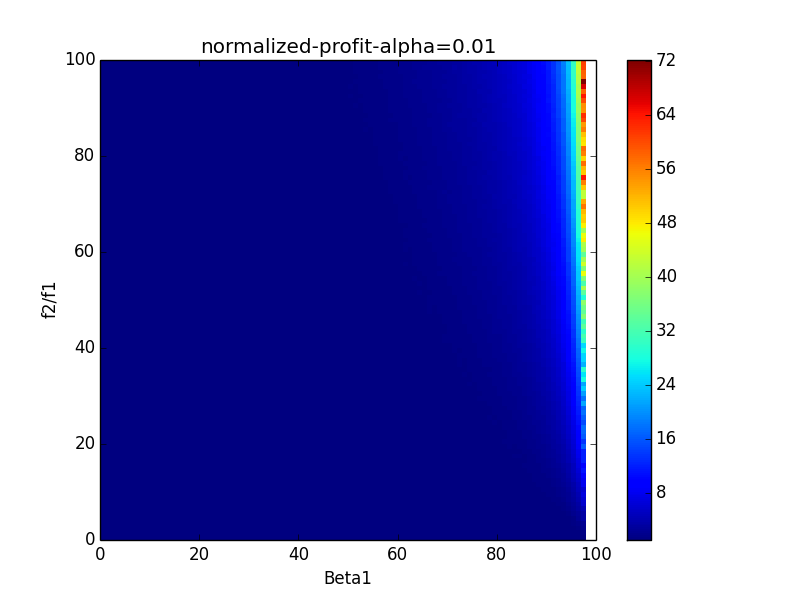
\includegraphics[width=0.25\linewidth]{simulations/resources/normalized-profit-alpha=0-01.png}
		\label{fig:theo}
		}
	\qquad
	\subfigure[$\alpha=0.05$]{
		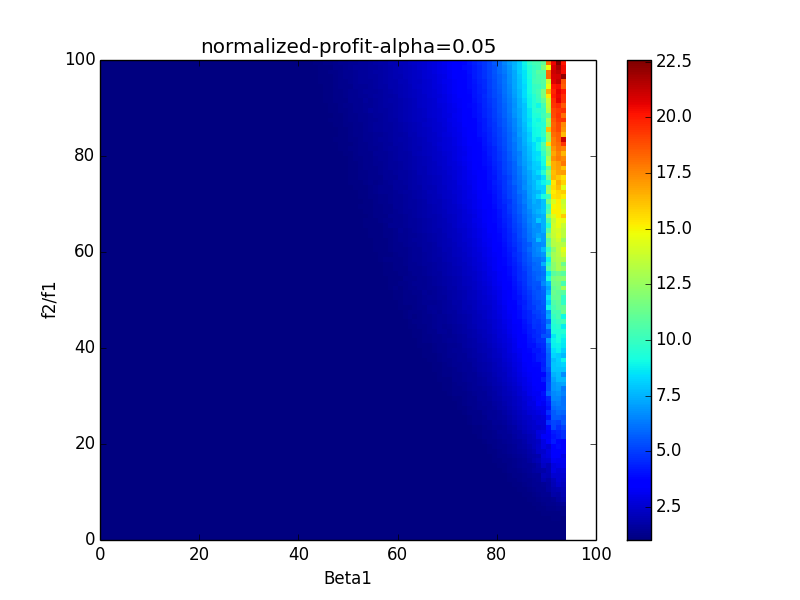
\includegraphics[width=0.25\linewidth]{simulations/resources/normalized-profit-alpha=0-05.png}
		\label{fig:theo}
		}
	\qquad
	\subfigure[$\alpha=0.1$]{
		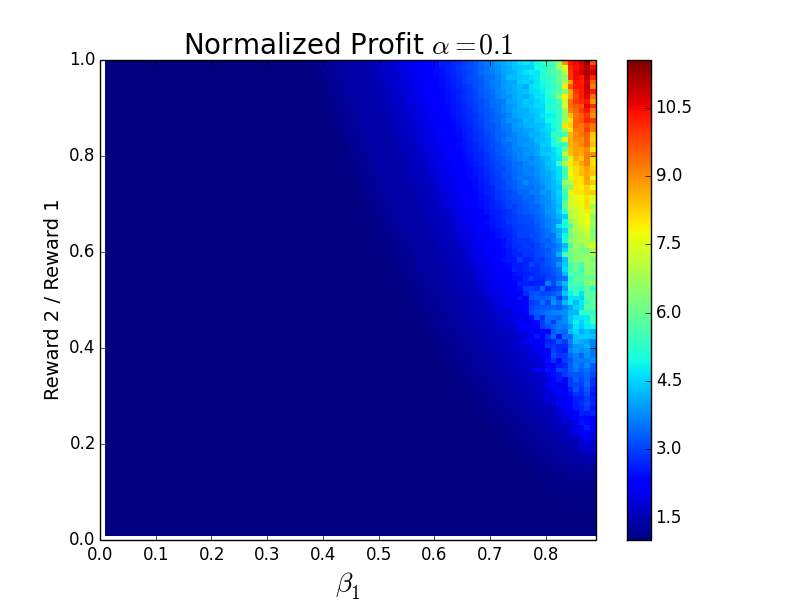
\includegraphics[width=0.25\linewidth]{simulations/resources/normalized-profit-alpha=0-1.png}
		\label{fig:theo}
		}
	\qquad
	\subfigure[$\alpha=0.2$]{
		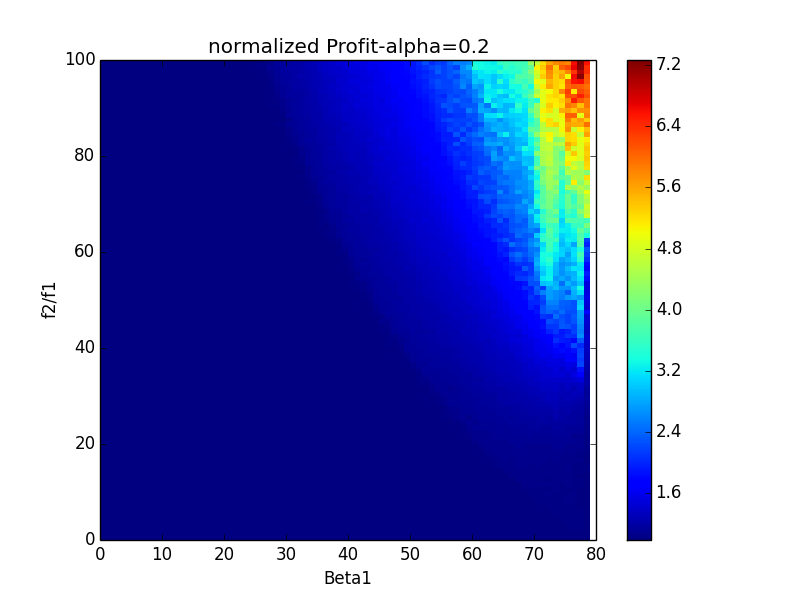
\includegraphics[width=0.25\linewidth]{simulations/resources/normalized-profit-alpha=0-2.png}
		\label{fig:theo}
		}
	\qquad
	\subfigure[$\alpha=0.3$]{
		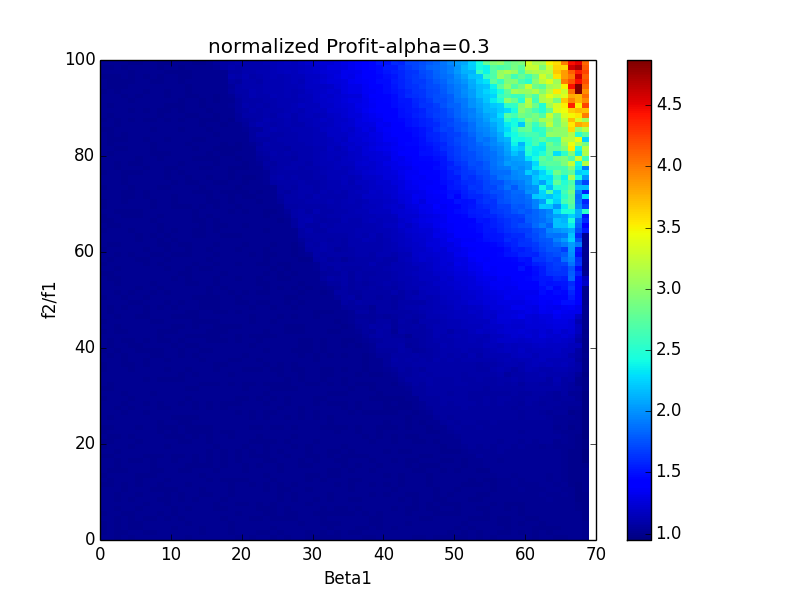
\includegraphics[width=0.25\linewidth]{simulations/resources/normalized-profit-alpha=0-3.png}
		\label{fig:theo}
		}		
	\caption{Normalized profitability of the greedy mercenary strategy.  This strategy is profitable throughout regions 2 and 3, and is relatively highest when chain 2's reward is relatively high and chain 2's loyal hash rate is relatively low.  Low total mercenary mining hash rate pays out relatively more than higher hash rates.}
\end{figure}

Figure 5 compares average time per block.  In general the lengthened block times of chains that have had their difficulty adjusted for but are then abandoned by mercenary miners outweigh the shortened block times in periods where the difficulty is not adjusted for mercenary miners.  This effect is visible in region 2.  As $\alpha$ increases the disruption in availability becomes more sever.
\begin{figure}
	\centering
	\subfigure[$\alpha=0.01$]{
		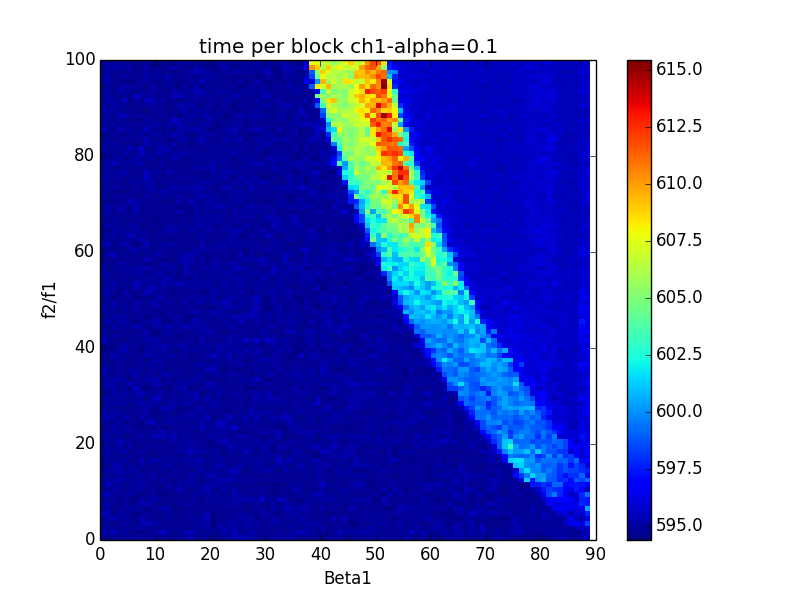
\includegraphics[width=0.25\linewidth]{simulations/resources/time-per-block-ch1-alpha=0-1.png}
		\label{fig:theo}
		}
	\qquad
	\subfigure[$\alpha=0.05$]{
		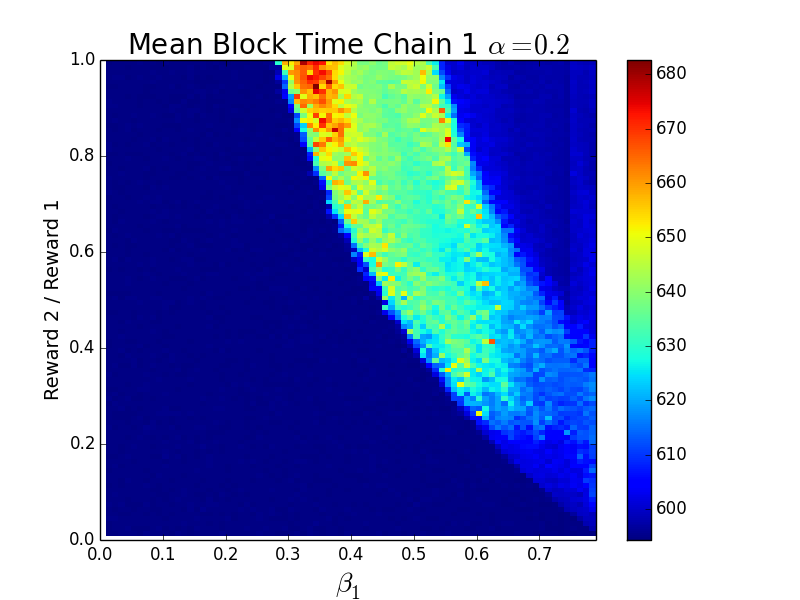
\includegraphics[width=0.25\linewidth]{simulations/resources/time-per-block-ch1-alpha=0-2.png}
		\label{fig:theo}
		}
	\qquad
	\subfigure[$\alpha=0.1$]{
		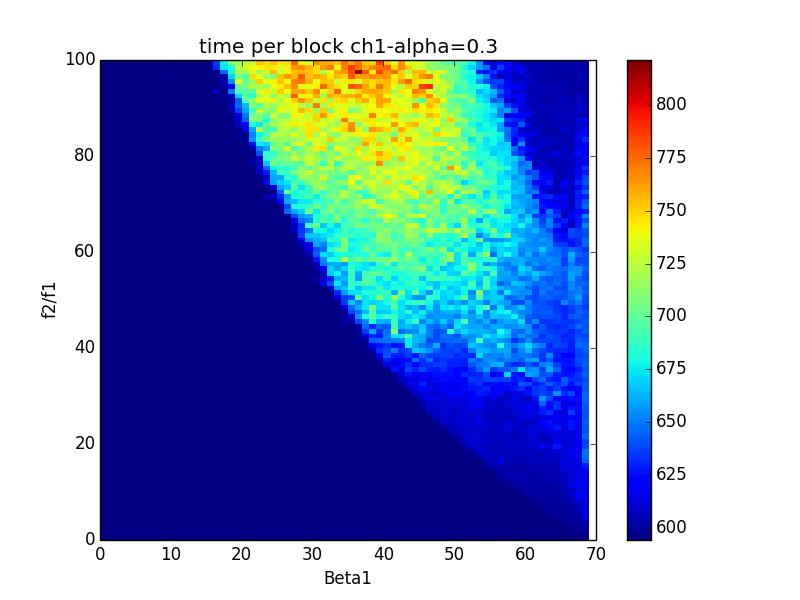
\includegraphics[width=0.25\linewidth]{simulations/resources/time-per-block-ch1-alpha=0-3.png}
		\label{fig:theo}
		}	
	\caption{Average block time.  Oscillations in mercenary hash power between chains on the whole decrease availability of the chains' transaction processing by slowing down block times on average.  The problem becomes more severe for higher $\alpha$}
\end{figure}


\section{Other Mercenary Strategies}
[TODO Ahaan is greedy optimal?]
[TODO Ahaan can you find a counter example?]


\section{A Competitive Protocol Leveraging Mercenaries}
One natural question following this analysis is whether a protocol could use the behavior of mercenary miners to its advantage when in competition with another chain.  This is interesting because new forks of more established protocols, such as the BCH fork of BTC, are often disadvantaged in terms of token exchange rate and total hash power but have the advantage of greater flexibility in defining new protocol rules.  These rules could potentially exploit the incentives of miners in two chain systems to become more advantaged along certain metrics.  Here we consider a simple technique in light of our understanding of the greedy mercenary miner strategy that could be used by such a competing blockchain protocol.  We begin by considering two metrics for which these networks might sensibly want to optimize.

A blockchain network has a vested interest in attracting a large share of the existing hash power applicable to its proof of work operating on its chain.  If hash power from a competing chain can be coordinated against a comparatively weaker chain then 51\% attacks and associated untrustworthy or unavailable transaction processing become a greater risk.  For this reason we consider the fraction of hash power out of the total pool of hash power relevant to the chain's proof of work to be a number that a protocol wishes to maximize.

Furthermore we hypothesize the rate at which a protocol specifies tokens are to be minted is a relevant metric.  The basic thinking is that if more tokens are mined then the markets for these tokens will see a decrease in value and the block reward's value will go down, creating a spiral where hashpower leaves a chain because miners find better profit elsewhere. We are not economists and recognize there is a great deal of complexity that could be explored here, but we'll assume throughout this section that the rate of tokens minted is something that chains would like to keep below some threshold.  The general structure of the technique outlined below should be useful even with a more complex optimization criterion for the minting rate.

\subsection{Getting the Best Deal}
The key idea behind our technique is that the hashpower of mercenary miners is effectively purchased by the protocol increasing its minting rate.  Mercenaries see more profit when difficulty is low on a chain and move their hashpower to this chain for the tradeoff of tokens of this chain being mined at a higher rate than before.  Another way to put this is that the expected profit rate calculation miners use to decide which chain to mine on is proportional to the minting rate of the chain.  Our technique is based on the following observation: mercenary miners in our model are incentivized to mine on the less powerful competing chain when its expected rate of profit is higher, however this chain could potentially push its expected rate of profit lower while maintaining incentive for the mercenaries to stay on its chain.  A chain using this technique would set its profit rate as low as possible, $\epsilon$ above the profit rate of the competing chain. 

To achieve this expected profit, and therefore minting, rate reduction a protocol has two options: raise the difficulty or reduce the token reward per block.  Raising the difficulty causes external effects that would likely harm the system's function, i.e. transaction throughput would be variably adjusted and hence unreliable.  Perhaps this is acceptable for a chain launching an attack against a stronger competitor as its primary purpose.  The alternate of modifying the coinbase token reward dynamically does not suffer from throughput reductions however, and it achieves the same purpose.  Note that to actually build a protocol that sets the profit rate this way, it is essential to measure the profit rate of the competing chain: $\frac{f_1}{d_1}$.  There is already a great way to get a value for $d_1$: the attacking protocol could maintain the competitor chain and measure directly from solutions to block puzzles.  Part of $f_1$ could be measured directly as well by looking at the coinbase transaction and fees of each block.  However the protocol itself would need to access an oracle for the values of the exchange rates of the two tokens.

In region 1 where chain 1 always controls the mercenaries, taking control of the $\alpha$ fraction of hash power requires raising the minting rate beyond the steady state of the protocol.

In region 2 chain 2 can lower its minting rate below the original steady state and still maintain control of the mercenary hash power.

In parts of region 3 chain 2 must raise its minting rate and in some parts it can lower its minting rate compared with the steady state to maintain control of mercenary hash power.

This can also be framed as "average mercenary hash power stolen given a fixed minting rate threshold" rather than "minting rate threshold given that mercenary hash power stays on chain 2 for all trials"

[TODO -- figure for clarifying first paragraph of this section ]
[TODO -- writing of the last part of this section]
[TODO -- Average merc hash power given a fixed minting rate thresh experiment results.  Modify simulations to have one chain use this protocol.  We'll have to start keeping track of coinbase values too now]


\section{Historical Analysis of Data}
[TODO Arnesh]


%The next switching point is influenced by the miner's choice of which chain to mine on.  Call 

\subsection{References}
[1] https://bitcoinandtheblockchain.blogspot.co.uk/2017/08/chain-death-spiral-fatal-bitcoin.html?m=1
[2] https://fork.lol/reward/dari/btc


\end{document}